% --------- Initialization ---------- % 
\documentclass[aspectratio=169]{beamer}
\usetheme{default}
\setbeamertemplate{navigation symbols}{}

% Packages
\usepackage{hyperref}
\definecolor{links}{HTML}{2A1B81}
\hypersetup{colorlinks,linkcolor=,urlcolor=links}
\usepackage{graphicx} 

% Personalise Font
\usefonttheme{professionalfonts} % using non standard fonts for beamer
\usefonttheme{serif}% default family is serif
\usepackage{mathpazo}

% Create Transitioning Slides at each section
\AtBeginSection[]{
	\begin{frame}
		\vfill
		\centering
		\begin{beamercolorbox}[sep=8pt,center,shadow=true,rounded=true]{title}
			\usebeamerfont{title}\insertsectionhead\par%
		\end{beamercolorbox}
		\vfill
	\end{frame}
}

% Miniframes Structure
\useoutertheme[subsection=false]{miniframes}
\makeatletter
\let\beamer@writeslidentry@miniframeson=\beamer@writeslidentry
\def\beamer@writeslidentry@miniframesoff{%
	\expandafter\beamer@ifempty\expandafter{\beamer@framestartpage}{}% does not happen normally
	{%else
		% removed \addtocontents commands
		\clearpage\beamer@notesactions%
	}
}
\newcommand*{\miniframeson}{\let\beamer@writeslidentry=\beamer@writeslidentry@miniframeson}
\newcommand*{\miniframesoff}{\let\beamer@writeslidentry=\beamer@writeslidentry@miniframesoff}


\title{Introduction to GitHub}
\author{Python-do-ECARES \\ Fabrizio Leone}
\date{}

% --------- Document stars here ----------- %
\begin{document}
\begin{frame}[plain]
    \maketitle
\end{frame}

% INTRO
\section{Introduction}

\begin{frame}{Git and GitHub}

\begin{itemize}\setlength\itemsep{2.5em}
	\item Git is a version control system, i.e. a way to keep track of the whole history of things you do on a file. It is useful to save, manage and edit all the different versions of your project. 
	\item GitHub is a web service that allows to conveniently work with Git. It allows you to create your own directories, see projects of other people and collaborate with them. 
	\item GitHub offers four different \href{https://github.com/pricing}{subscription plans}. We will work with a free one, which means that \emph{everybody} can see what we do. However, with an academic account, you can also create private repositories.
\end{itemize}

\end{frame}

\begin{frame}{GitHub: What It Does And Does Not Do}
\begin{itemize}\setlength\itemsep{2.0em}
	\item No matter which subscription plan you choose, GitHub offers very limited storage space (you cannot upload files $>100$MB). Therefore, it is \textbf{not} suitable for storing large files (e.g. datasets). \textbf{GitHub is not a substitute for a cloud}.  
	\item GitHub is a platform where to upload mostly \textbf{source files} (e.g. .tex, .txt, .m, .R, .do, .py, .doc,...) and light pdf.
	\item You can read more about Git and GitHub \href{https://medium.com/@abhishekj/an-intro-to-git-and-github-1a0e2c7e3a2f}{here} and \href{https://medium.com/launch-school/understanding-git-and-github-8ac987877a5}{here}.
\end{itemize}

\end{frame}

\begin{frame}{GitHub Desktop}

\begin{itemize}\setlength\itemsep{2em}
		\item In this course, we interact with GitHub mostly through the GitHub Desktop application.
		\item GitHub Desktop provides a simple yet powerful desktop interface to GitHub.
		\item You can download GitHub desktop \href{https://desktop.github.com/}{here}. 
		\item You can also interact with GitHub using the \href{https://github.com/codepath/ios_guides/wiki/Using-Git-with-Terminal}{Terminal} (not covered in this class).
\end{itemize}	

\end{frame}

% GitHub Desktop
\section{First Steps With GitHub Desktop}

\begin{frame}{Step 1. Clone Repository}{Go to the \href{https://github.com/Python-do-ECARES/Classes}{Classes} repository on GitHub and click on the "Clone or download" button.}
\begin{figure}
	\centering
	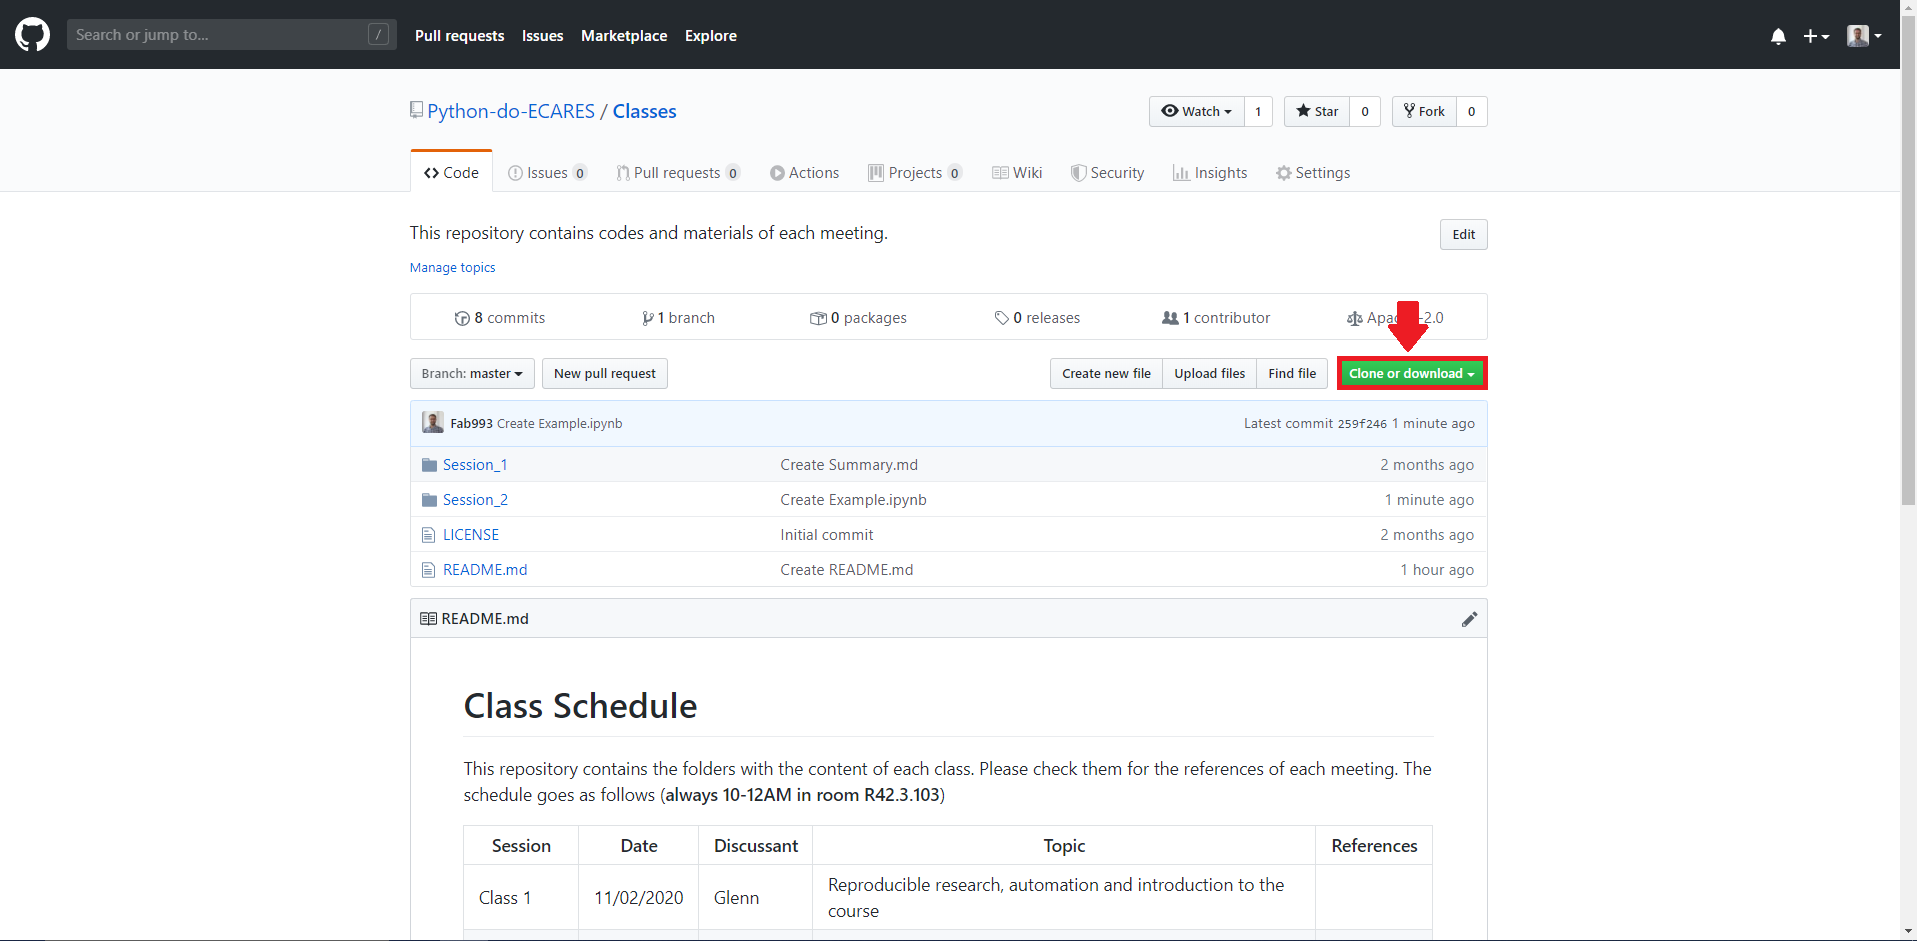
\includegraphics[width=0.9\linewidth]{../images/step1}
\end{figure}
\end{frame}

\begin{frame}{Step 1.A Open Repository}{Choose "Open in Desktop".}	
	\begin{figure}
		\centering
		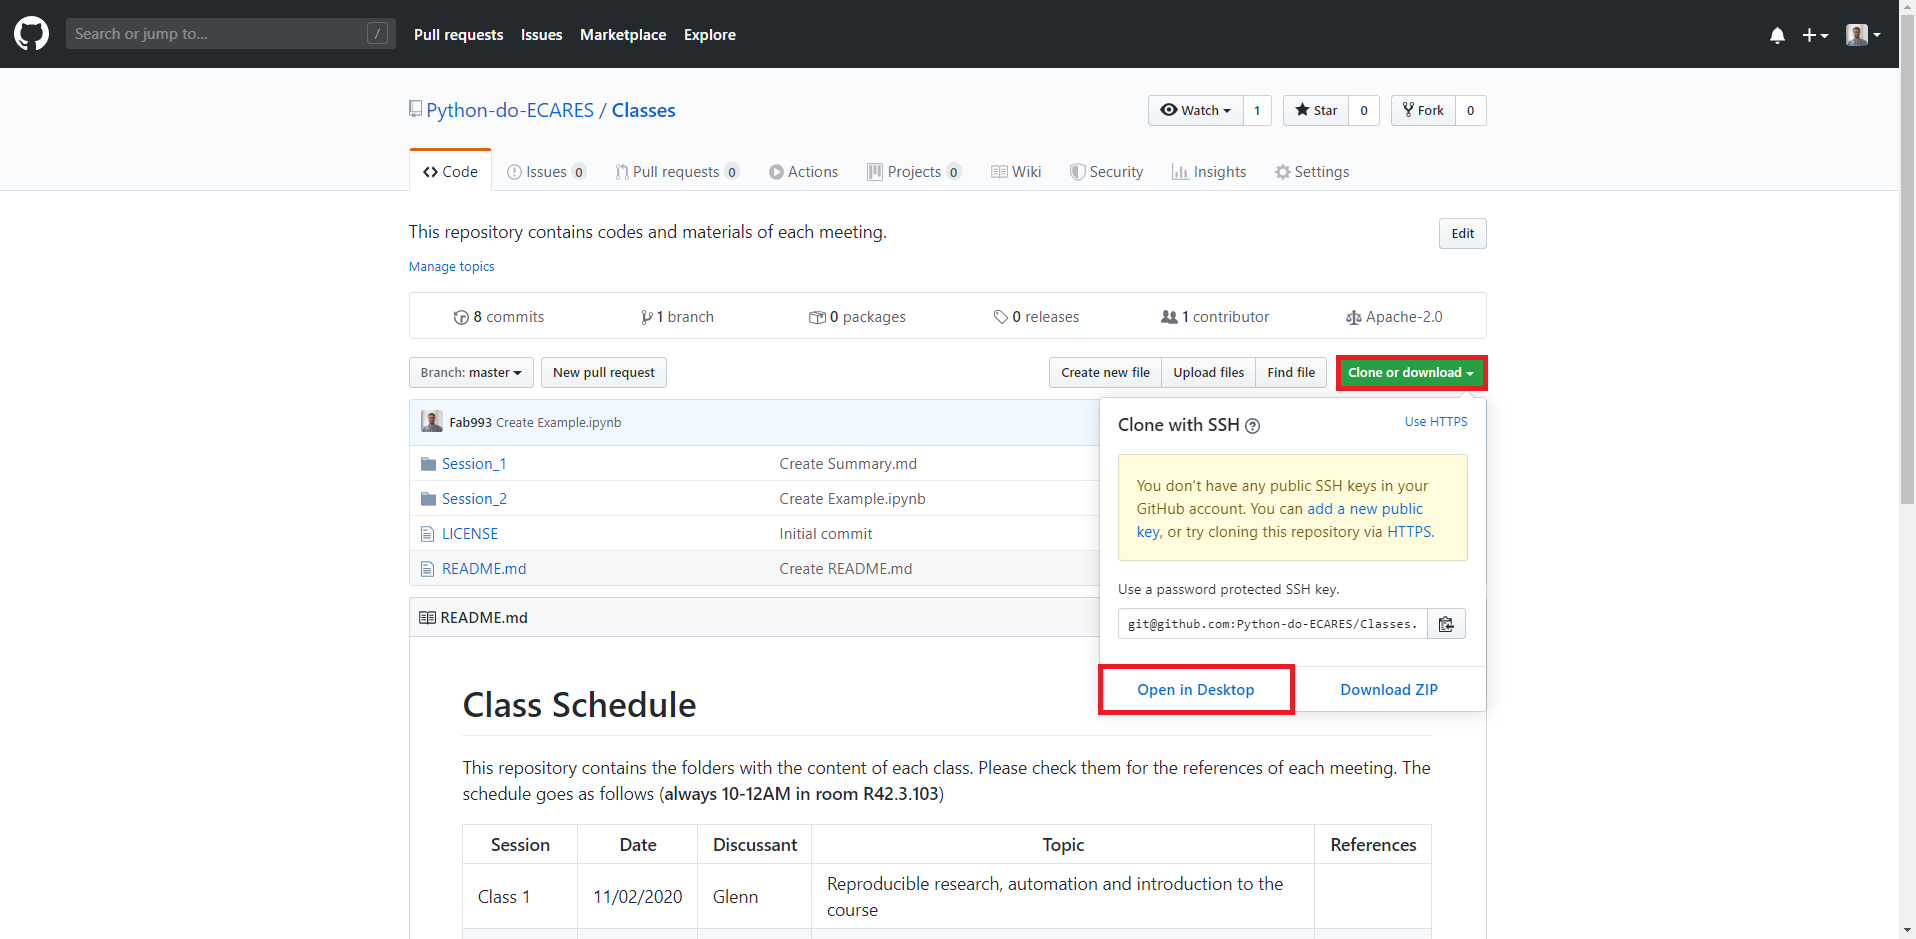
\includegraphics[width=0.9\linewidth]{../images/step1.A}
	\end{figure}
\end{frame}

\begin{frame}{Step 1.B Clone Repository}{Check the local path where to clone the repository and click "Clone".}
	\begin{figure}
		\centering
		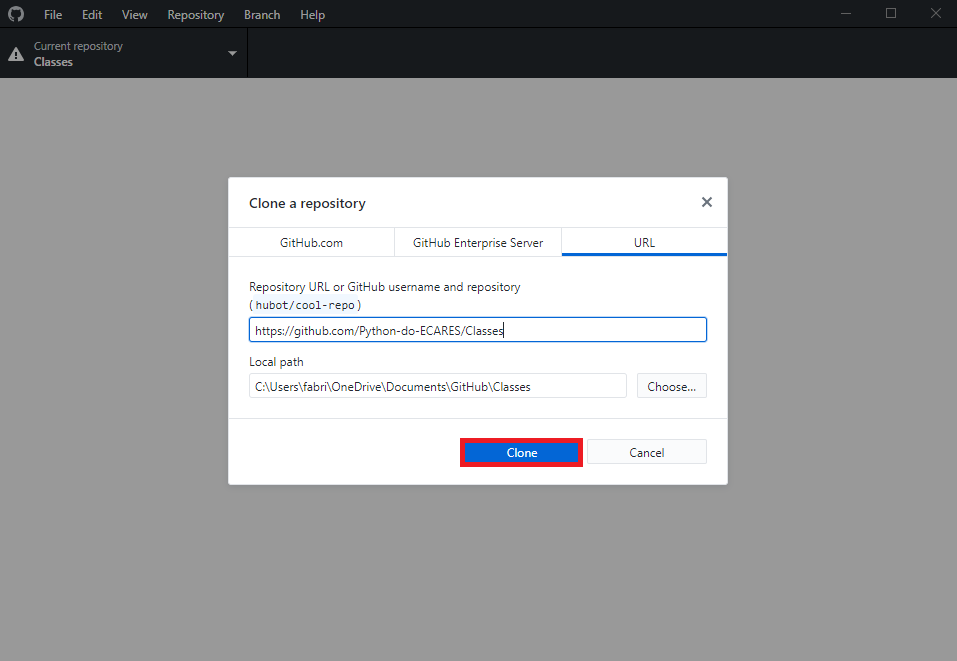
\includegraphics[width=0.7\linewidth]{../images/step1.B}
	\end{figure}
\end{frame}

\begin{frame}{Step 1.C Open Local Directory}{Under GitHub Desktop/Classes/Session$\_2$ you will see the following files.}
	\begin{figure}
		\centering
		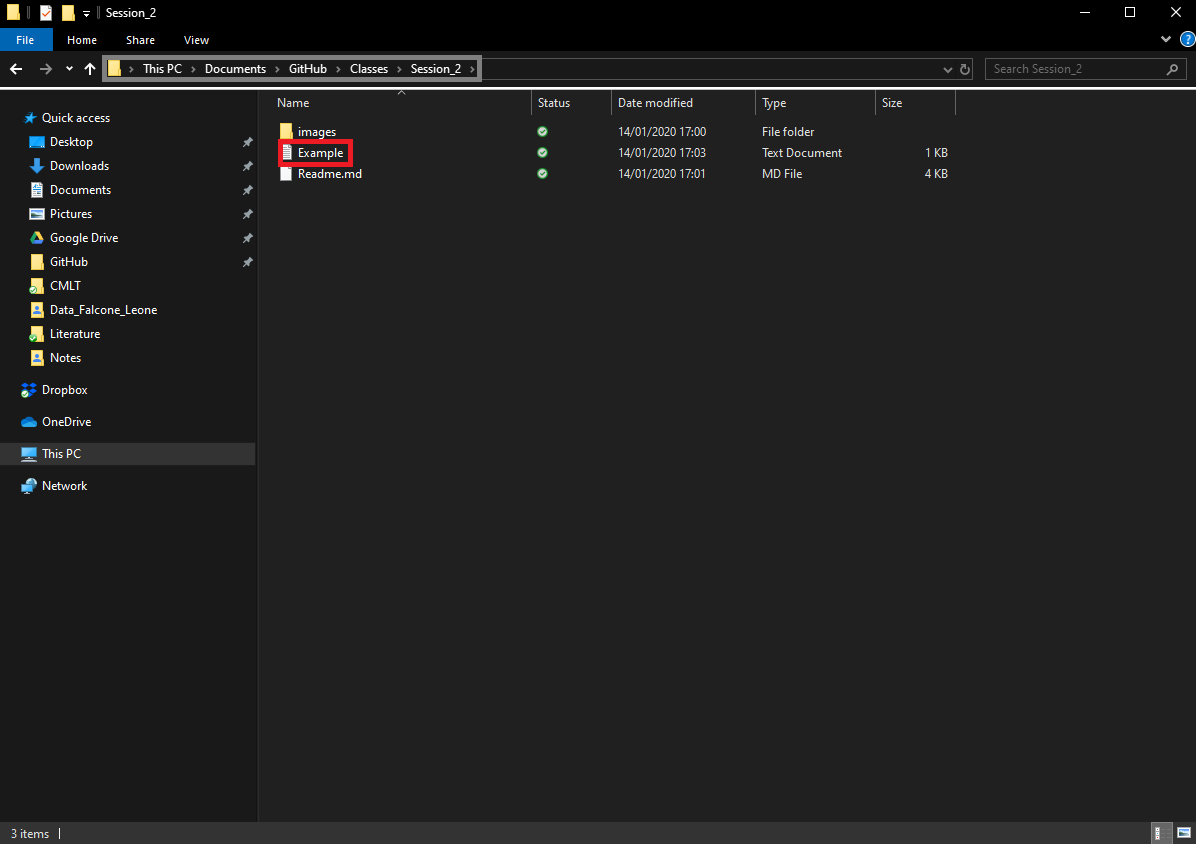
\includegraphics[width=0.7\linewidth]{../images/step1.C}
	\end{figure}
\end{frame}

\begin{frame}{Step 2 Make Changes}{Open \emph{Example.txt}. Add a comment line with your name.}
	\begin{figure}
		\centering
		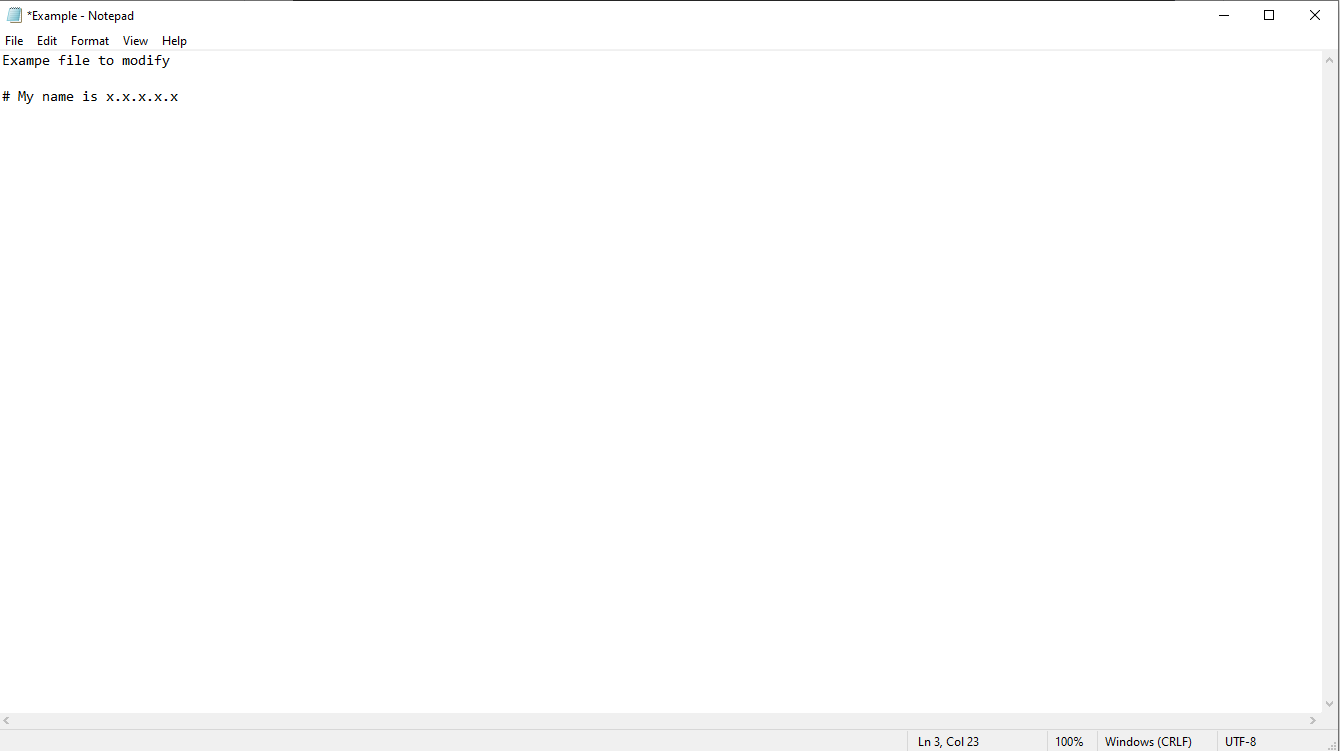
\includegraphics[width=0.8\linewidth]{../images/step2}
	\end{figure}
\end{frame}

\begin{frame}{Step 2.A Save Changes}{Save the file. Changes will be displayed in GitHub Desktop as follows.}
	\begin{figure}
		\centering
		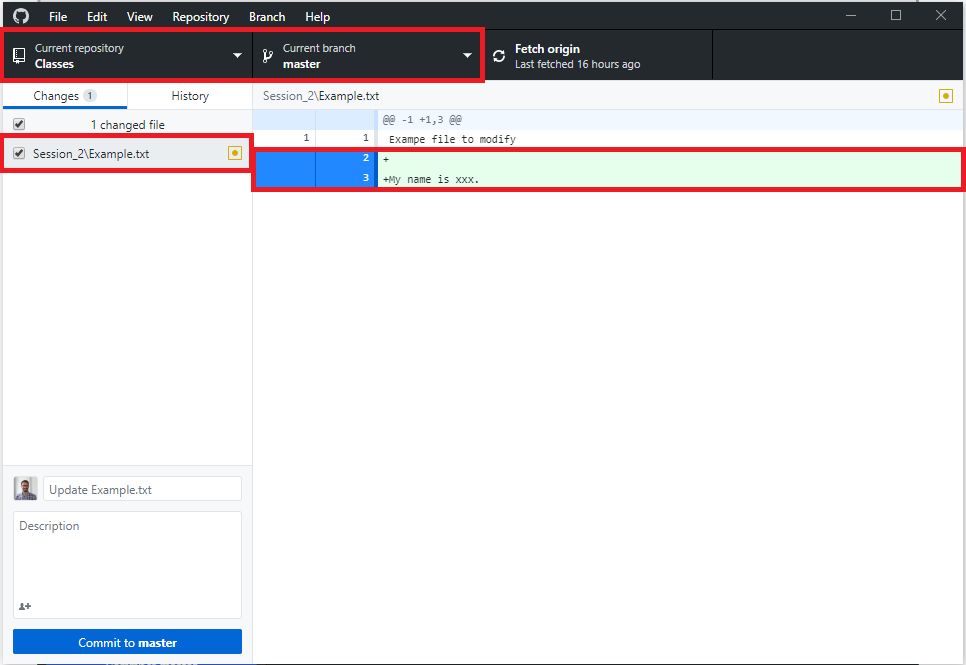
\includegraphics[width=0.7\linewidth]{../images/step2.A}
	\end{figure}
\end{frame}

\begin{frame}{Step 2.B Create Your Own Branch And Commit Changes}{Select "Master" and "New Branch". Never directly commit your changes to the Master during this course.}
	\begin{figure}
		\centering
		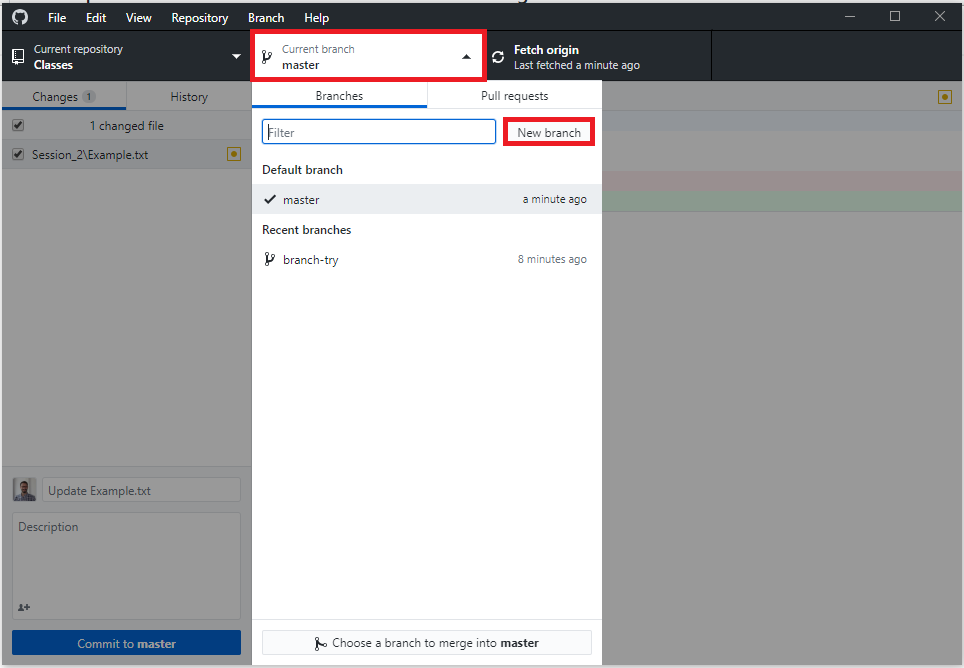
\includegraphics[width=0.7\linewidth]{../images/step2.B}
	\end{figure}
\end{frame}


\begin{frame}{Step 2.C Name Branch}{Give the new branch your name. Then click "Create Branch".}
	\begin{figure}
		\centering
		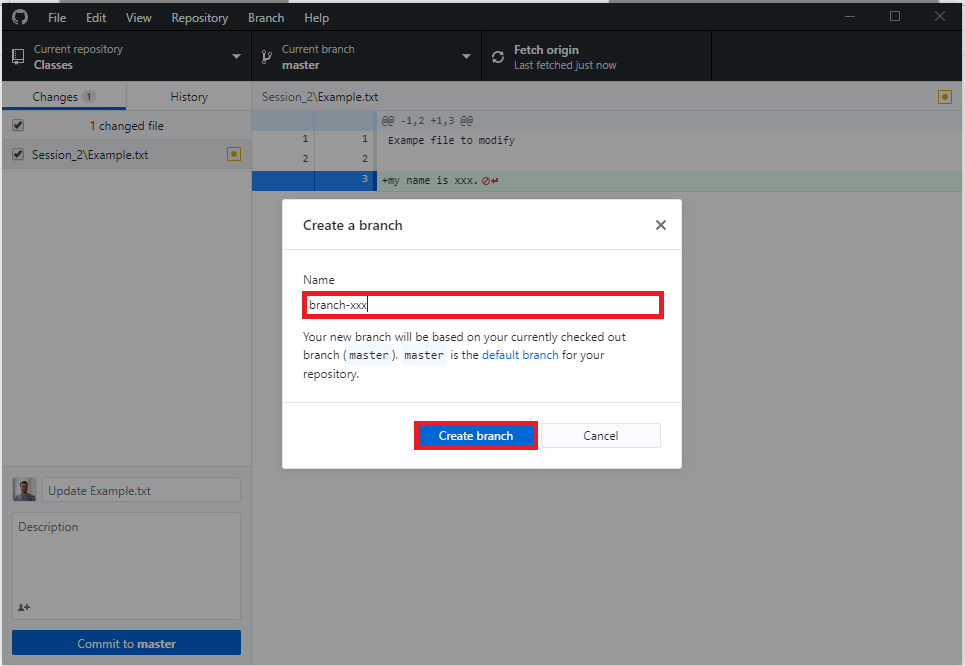
\includegraphics[width=0.7\linewidth]{../images/step2.C}
	\end{figure}
\end{frame}

\begin{frame}{Step 2.D Switch Branch}{Switch changes to your own branch.}
	\begin{figure}
		\centering
		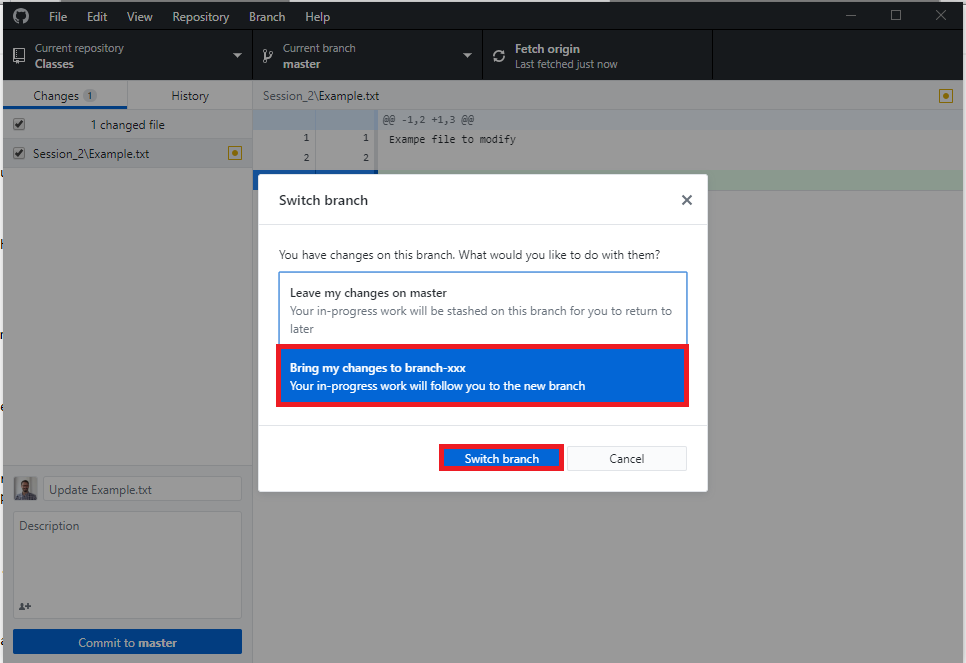
\includegraphics[width=0.7\linewidth]{../images/step2.D}
	\end{figure}
\end{frame}

\begin{frame}{Step 2.E Publish Branch}{Publish your branch online.}
	\begin{figure}
		\centering
		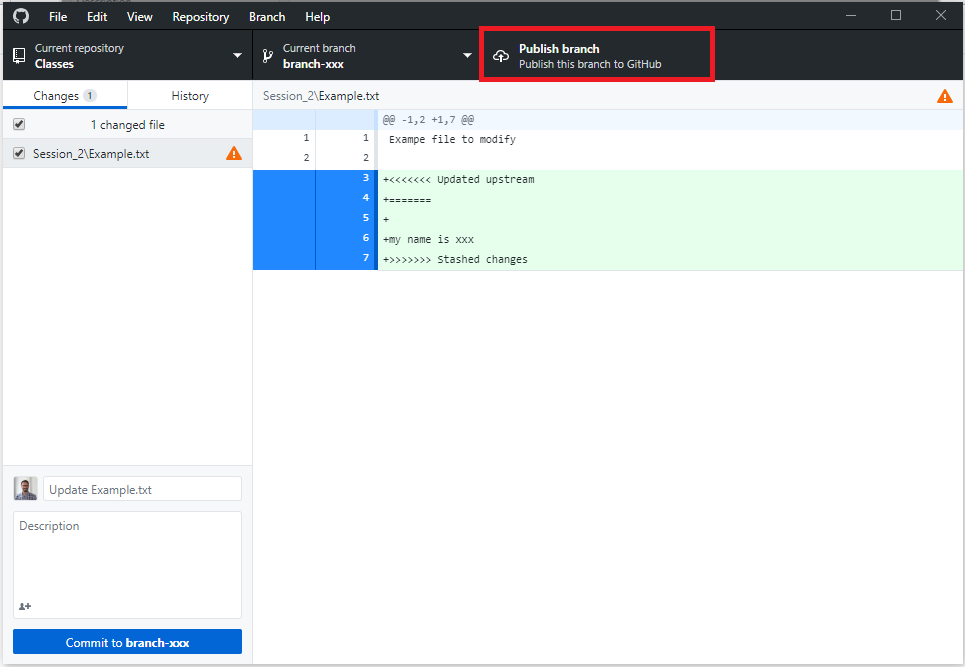
\includegraphics[width=0.7\linewidth]{../images/step2.E}
	\end{figure}
\end{frame}

\begin{frame}{Step 2.E Commit to Branch}{Give Description and summary. Then commit.}
	\begin{figure}
		\centering
		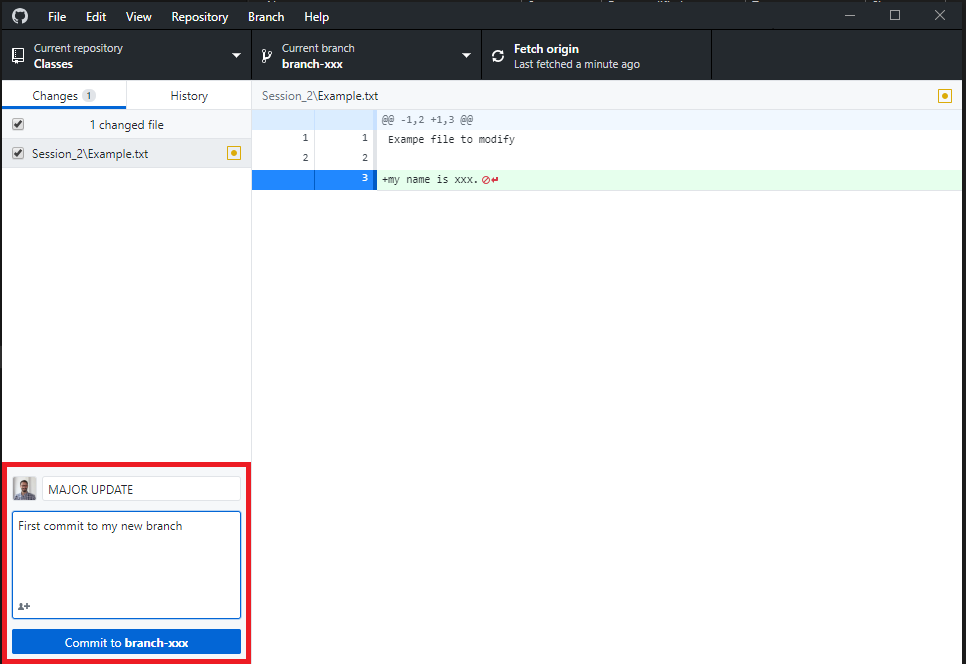
\includegraphics[width=0.7\linewidth]{../images/step2.F}
	\end{figure}
\end{frame}


\begin{frame}{Step 2.E Push to Branch}{Push changes to your branch.}
	\begin{figure}
		\centering
		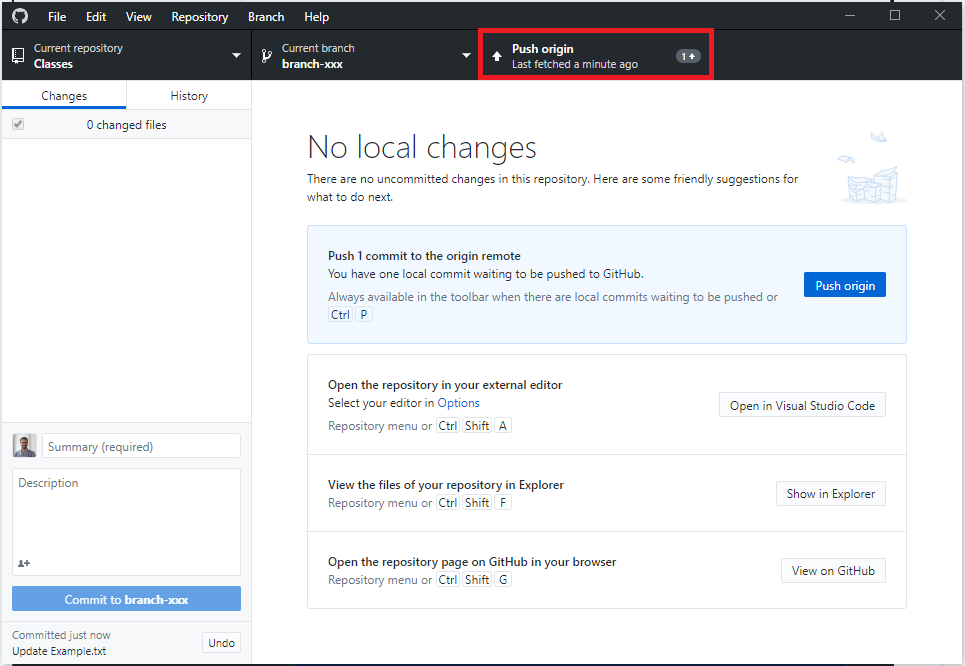
\includegraphics[width=0.7\linewidth]{../images/step2.G}
	\end{figure}
\end{frame}


\begin{frame}{Step 3 Next Steps}{Go to "Classes" page. Notice that now there are 2 branches. Click on "branches".}
	\begin{figure}
		\centering
		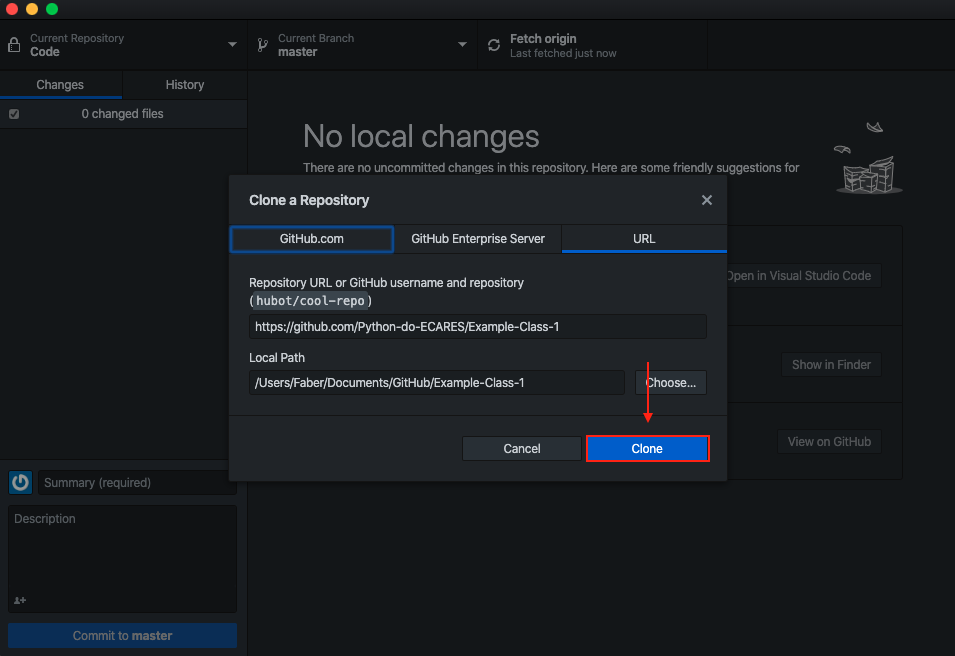
\includegraphics[width=0.9\linewidth]{../images/step3}
	\end{figure}
\end{frame}

\begin{frame}{Step 3.A Done!}{Your directory will now appear below "branches" as follows.}
	\begin{figure}
		\centering
		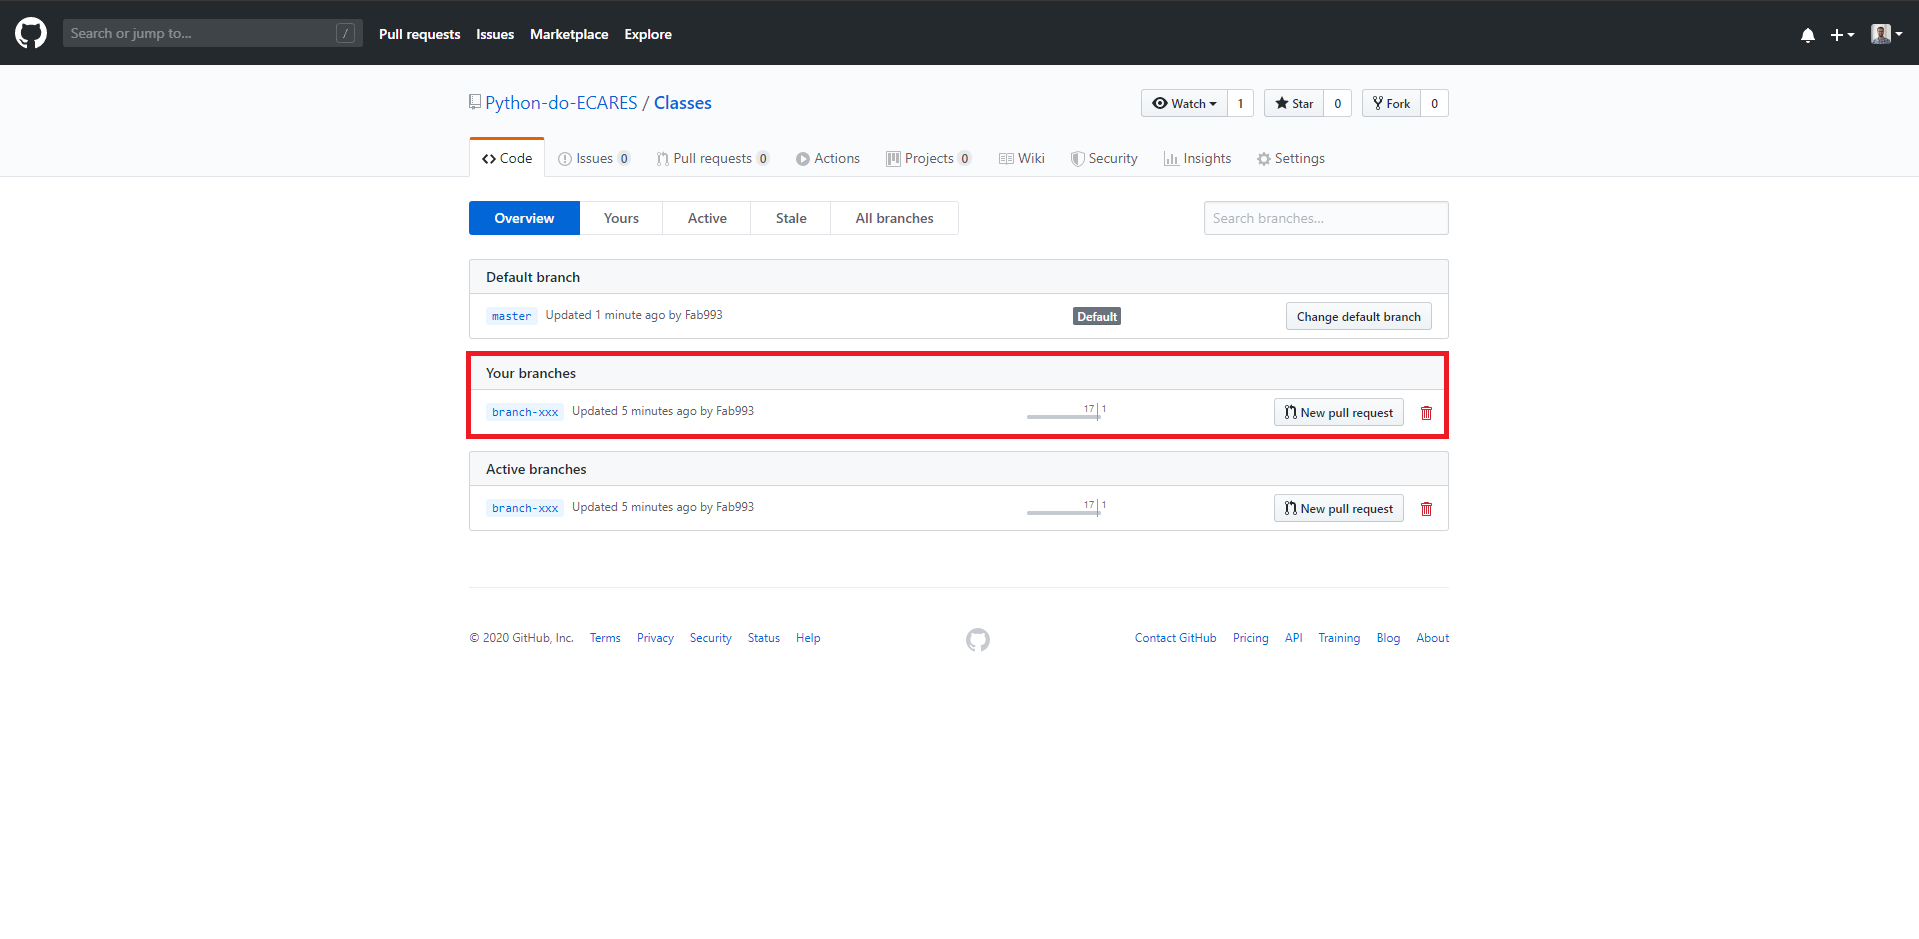
\includegraphics[width=1\linewidth]{../images/step3.A}
	\end{figure}
\end{frame}

\begin{frame}{Taking Stocks}
\begin{itemize}\setlength\itemsep{2.5em}
	\item You are now able to create and maintain \textbf{your own repositories}.
	\item Please \textbf{make sure your only push changes to your own branch during this course}. You are encouraged to collaborate and see what other people is up to, but \textbf{never} commit changes directly to other people's branches.
	\item Good news is that you can always revert changes back if you do so by mistake. This is why GitHub is so useful!
\end{itemize}
\end{frame}

% Commit and Push
\section{Commit and Push}

\begin{frame}{Commit and Push}
	\begin{itemize}\setlength\itemsep{1.5em}
		\item \textbf{Committing} and \textbf{pushing} are the main two words you have to familiarize with.
		\item \emph{Committing changes} to a branch, means that you are "saving" your changes.
		\item \emph{Pushing changes} means, instead, that you are publishing them online on GitHub.Think of the pushing action as a way of creating different stable releases of your code.\item With this respect, we recomment to commit changes regurlarly (you can always revert them back), but to only push them online if you have made a stable change. 
	\end{itemize}
\end{frame}

\begin{frame}{Social Norms}
	\begin{itemize}\setlength\itemsep{2.5em}
		\item We encourage you to adopt the following standards to commit and push tidely.
		\item Summary should be either\textbf{ Minor Change}, \textbf{Major Change} or \textbf{Bug Fixes}. The first should indicate small changes in syntaxis or general improvements. The second to major modifications (e.g. add new section or function), while the third is to notify that you have fixed some bug.
		\item \textbf{Description} should briefly explain what the summary refers to.
	\end{itemize}
\end{frame}

\begin{frame}{Social Norms}
	\begin{itemize}\setlength\itemsep{2.5em}
		\item Suppose you \textbf{create a new function for data cleaning in your code}. When pushing this change to GitHub, you want to give\textbf{Major Change} as summary and "added function for data cleaning" as description.
		\item A tidy pushing activities will create a full history of changes in GitHub that you can scroll through to check different versions of your code.
		\item Finally, it will also help other people to understand your work.
	\end{itemize}
\end{frame}

% Browse through history
\section{Browse Through History}

\begin{frame}{Browse Through History}
	With GitHub Desktop, you can also browse through the entire history of your commits. This is very helpful to \vspace{1cm}
		\begin{itemize}\setlength\itemsep{2.5em}
		\item \textbf{Revert back changes}. Imagine you update a code but, at some point, you realise that one of the previous releases was better. 
		\item \textbf{Compare different versions}. From time to time, you may want to look back at previous versions of your work (slide, paper, code,...).
	\end{itemize}
\end{frame}


\end{document}
